\documentclass[11pt]{article}

%% PACKAGES
\usepackage{graphicx}
\usepackage[printonlyused]{acronym}
\usepackage{float}
\usepackage[colorlinks=false]{hyperref}
\usepackage{tabularx}
\usepackage{caption}
\usepackage[margin=1.0in]{geometry}
\usepackage{tocloft}
\usepackage{listings}

\lstset{basicstyle=\small\ttfamily,columns=flexible,breaklines=true,xleftmargin=0.5in,keepspaces=true}


\makeatletter
\g@addto@macro\normalsize{%
  \setlength\abovedisplayskip{0.25pt}
  \setlength\belowdisplayskip{0.25pt}
  \setlength\abovedisplayshortskip{0.25pt}
  \setlength\belowdisplayshortskip{0.25pt}
}
\makeatother

\setlength{\parskip}{\baselineskip}

%% GRAPHICS PATH
\graphicspath{{../../../shared_latex_inputs/images}{../../../shared_latex_inputs/graphs}}

\newcommand{\acposs}[1]{%
	\expandafter\ifx\csname AC@#1\endcsname\AC@used
	\acs{#1}'s%
	\else
	\aclu{#1}'s (\acs{#1}'s)%
	\fi
}

\title{\Huge EMTG Tutorial: Flybys}
\vspace{0.5cm}
\author
{
	Tim Sullivan \thanks{Aerospace Engineer, The Aerospace Corporation}
}
\vspace{0.5cm}

\newcommand{\listofknownissuesname}{\Large List of Known Issues}
\newlistof{knownissues}{mcf}{\listofknownissuesname}

\newcommand{\knownissue}[3]
{
	\refstepcounter{knownissues}
	\par\noindent\textbf{\hyperref[#2_b]{\theknownissues\quad #1}}\label{#2_h}
	\textbf{\hfill\pageref{#2_b}}
	#3
}

\newcommand{\knownissuelabel}[2]
{
	 \phantomsection
  	\hyperref[#2_h]{#1}\def\@currentlabel{\unexpanded{#1}}\label{#2_b}
}


\begin{document}

\begin{titlepage}
\maketitle
\thispagestyle{empty}
\begin{table}[H]
	\centering
	\begin{tabularx}{\textwidth}{|l|l|X|}
		\hline
		\textbf{Revision Date} & \textbf{Author} & \textbf{Description of Change} \\
		\hline
		\date{December 2, 2022} & Tim Sullivan & Initial revision.\\
		\hline
		\date{June 30, 2023} & Joseph Hauerstein & Conversion to \LaTeX.\\ 
		\hline
		\date{August 4, 2023} & Joseph Hauerstein & Addition of Known Issues section.\\ 
		\hline
	\end{tabularx}
\end{table}
\end{titlepage}

\newpage
\tableofcontents
\thispagestyle{empty}
\newpage

\listofknownissues
\thispagestyle{empty}

\knownissue{Bug opening EMTG options file in text editor using PyEMTG}{text_editor_issue}

\newpage
\clearpage
\setcounter{page}{1}



%\section*{List of Acronyms}
\begin{acronym}
%To define the acronym and include it in the list of acronyms: \acro{acronym}{definition}
%To define the acronym and exclude it from the list of acronyms:  \acro{acronym}{definition}
%
%\ac{acronym} Expand and identify the acronym the first time; use only the acronym thereafter
%\acf{acronym} Use the full name of the acronym.
%\acs{acronym} Use the acronym, even before the first corresponding \ac command
%\acl{acronym}  Expand the acronym without using the acronym itself.
%
%

\acro{TCM}{trajectory correction maneuver}
\acro{ACO}{Ant Colony Optimization}
\acro{AD}{Automatic Differentiation}
\acro{ADL}{Architecture Design Laboratory}
\acro{ADM}{asteroid departure maneuver}
\acro{AEI}{atmospheric entry interface}
\acro{AES}{Advanced Exploration Systems}
\acro{AGA}{aerogravity assist}
\acro{ALARA}{As Low As Reasonably Achievable}
\acro{API}{application programming interface}
\acro{BB}{branch and bound}
\acro{BVP}{Boundary Value Problem}
\acro{CATO}{Computer Algorithm for Trajectory Optimization}
\acro{CL}{confidence level}
\acro{CONOPS}{concept of operations}
\acro{COV}{Calculus of Variations}
\acro{D/AV}{Descent/Ascent Vehicle}
\acro{DE}{Differential Evolution}
\acro{RLA}{Right Ascension of Launch Asymptote}
\acro{DLA}{Declination of Launch Asymptote}
\acro{DPTRAJ/ODP}{Double Precision Trajectory and Orbit Determination Program}
\acro{DSH}{Deep Space Habitat}
\acro{DSN}{Deep Space Network}
\acro{DSMPGA}{Dynamic-Size Multiple Population Genetic Algorithm}
\acro{EB}{Evolutionary Branching}
\acro{ECLSS}{environmental control and life support system}
\acro{EGA}{Earth gravity assist}
\acro{ELV}{expendable launch vehicle}
\acro{EMME}{Earth to Mars, Mars to Earth}
\acro{EMMVE}{Earth to Mars, Mars to Venus to Earth}
\acro{EMTG}{Evolutionary Mission Trajectory Generator}
\acro{EVMME}{Earth to Venus to Mars, Mars to Earth}
\acro{EVMMVE}{Earth to Venus to Mars, Mars to Venus to Earth}
\acro{ERRV}{Earth Return Re-entry Vehicle}
\acro{FISO}{Future In-Space Operations}
\acro{FMT}{Fast Mars Transfer}
\acro{GASP}{Gravity Assist Space Pruning}
\acro{GCR}{galactic cosmic radiation}
\acro{GRASP}{Greedy Randomized Adaptive Search Procedure}
\acro{GSFC}{Goddard Space Flight Center}
\acro{GTOC}{Global Trajectory Optimization Competition}
\acro{GTOP}{Global Trajectory Optimization Problem}
\acro{HAT}{Human Architecture Team}
\acro{HGGA}{Hidden Genes Genetic Algorithm}
\acro{IMLEO}{Initial Mass in \acl{LEO}}
\acro{IPOPT}{Interior Point OPTimizer}
\acro{ISS}{International Space Station}
\acro{JHUAPL}{Johns Hopkins University Applied Physics Laboratory}
\acro{JSC}{Johnson Space Center}
\acro{KKT}{Karush-Kuhn-Tucker}
\acro{LEO}{Low Earth Orbit}
\acro{LRTS}{lazy race tree search}
\acro{MAT}{Mars Architecture Team}
\acro{MONTE}{Mission analysis, Operations, and Navigation Toolkit Environment}
\acro{MCTS}{Monte Carlo tree search}
\acro{MGA}{Multiple Gravity Assist}
\acro{MIRAGE}{Multiple Interferometric Ranging Analysis using GPS Ensemble}
\acro{MOGA}{Multi-Objective Genetic Algorithm}
\acro{MOSES}{Multiple Orbit Satellite Encounter Software}
\acro{MPI}{message passing interface}
\acro{MPLM}{Multi-Purpose Logistics Module}
\acro{MSFC}{Marshall Space Flight Center}
\acro{NELLS}{NASA Exhaustive Lambert Lattice Search}
\acro{NMDB}{Navigation and Mission Design Branch}
\acro{NSGA}{Non-Dominated Sorting Genetic Algorithm}
\acro{NSGA-II}{Non-Dominated Sorting Genetic Algorithm II}
\acro{NHATS}{Near-Earth Object Human Space Flight Accessible Targets Study}
\acro{NTP}{Nuclear Thermal Propulsion}
\acro{OD}{orbit determination}
\acro{OOS}{On-Orbit Staging}
\acro{PCC}{Pork Chop Contour}
\acro{PEL}{permissible exposure limits}
\acro{PLATO}{PLAnetary Trajectory Optimization}
\acro{REID}{risk of exposure-induced death}
\acro{RTBP}{Restricted Three Body Problem}
\acro{SA}{Simulated Annealing}
\acro{SLS}{Space Launch System}
\acro{SNOPT}{Sparse Nonlinear OPTimizer}
\acro{SOI}{sphere of influence}
\acro{SPE}{solar particle events}
\acro{SQP}{sequential quadratic programming}
\acro{SRAG}{Space Radiation Analysis Group}
\acro{TEI}{Trans-Earth Injection}
\acro{TIM}{technical interchange meeting}
\acro{TOF}{time of flight}
\acro{TPBVP}{Two Point Boundary Value Problem}
\acro{TMI}{Trans-Mars Injection}
\acro{VARITOP}{Variational calculus Trajectory Optimization Program}
\acro{VGA}{Venus gravity assist}
\acro{VILM}{v-infinity leveraging maneuver}
\acro{MOI}{Mar Orbit Injection}
\acro{PCM}{Pressurized Cargo Module}
\acro{STS}{Space Transportation System}
\acro{EDS}{Earth Departure Stage}
\acro{NEO}{near-Earth asteroid}
\acro{IDC}{Integrated Design Center}
\acro{SEP}{solar-electric propulsion}
\acro{SRP}{solar radiation pressure}
\acro{NEP}{nuclear-electric propulsion}
\acro{REP}{radioisotope-electric propulsion}
\acro{DRM}{Design Reference Missions}

\acro{ASCII}{American Standard Code for Information Interchange}
\acro{AU}{Astronomical Unit}
\acro{BWG}{Beam Waveguides}
\acro{CCB}{Configuration Control Board}
\acro{CMO}{Configuration Management Office}
\acro{CODATA}{Committee on Data for Science and Technology}
\acro{DEEVE}{Dynamically Equivalent Equal Volume Ellipsoid}
\acro{DRA}{Design Reference Asteroid}
\acro{EME2000}{Earth Centered, Earth Mean Equator and Equinox of J2000 (Coordinate Frame)}
\acro{EOP}{Earth Orientation Parameters}
\acro{ET}{Ephemeris Time}
\acro{FDS}{Flight Dynamics System}
\acro{FTP}{File Transfer Protocol}
\acro{GSFC}{Goddard Space Flight Center}
\acro{PI}{Principal Investigator}
\acro{HEF}{High Efficiency}
\acro{IAG}{International Association of Geodesy}
\acro{IAU}{International Astronomical Union}
\acro{IERS}{International Earth Rotation and Reference Systems Service}
\acro{ICRF}{International Celestial Reference Frame}
\acro{ITRF}{International Terrestrial Reference System}
\acro{IOM}{Interoffice Memorandum}
\acro{JD}{Julian Date}
\acro{JPL}{Jet Propulsion Laboratory}
\acro{LM}{Lockheed Martin}
%\acro{LP150Q}{}
%\acros{LP100K}{}
\acro{MAVEN}{Mars Atmosphere and Volatile EvolutioN}
\acro{MJD}{Modified Julian Date}
\acro{MOID}{Minimum Orbit Intersection Distance}
\acro{MPC}{Minor Planet Center}
\acro{NASA}{National Aeronautics and Space Administration}
\acro{NDOSL}{\ac{NASA} Directory of Station Locations}
\acro{NEA}{near-Earth asteroid}
\acro{NEO}{near-Earth object}
\acro{NIO}{Nav IO}
\acro{OSIRIS-REx}{Origins, Spectral Interpretation, Resource Identification, and Security-Regolith Explorer}
\acro{PHA}{Potentially Hazardous Asteroid}
\acro{PHO}{Potentially Hazardous Object}
\acro{SBDB}{Small-Body Database}
\acro{SI}{International System of Units}
\acro{SPICE}{Spacecraft Planet Instrument Camera-matrix Events}
\acro{SPK}{SPICE Kernel}
\acro{SRC}{Sample Return Capsule}
\acro{SSD}{Solar System Dynamics}
\acro{AGI}{Analytical Graphics, Inc.}
\acro{STK}{Systems Tool Kit}
\acro{TAI}{International Atomic Time}
\acro{TBD}{To Be Determined}
\acro{TBR}{To Be Reviewed}
\acro{TCB}{Barycentric Coordinate Time}
\acro{TDB}{Temps Dynamiques Barycentrique, Barycentric Dynamical Time}
\acro{TDT}{Terrestrial Dynamical Time}
\acro{TT}{Terrestrial Time}
\acro{URL}{Uniform Resource Locator}
\acro{UT}{Universal Time}
\acro{UT1}{Universal Time Corrected for Polar Motion}
\acro{UTC}{Coordinated Universal Time}
\acro{USNO}{U. S. Naval Observatory}
\acro{YORP}{Yarkovsky-O'Keefe-Radzievskii-Paddack}

\acro{NLP}{nonlinear program}
\acro{MBH}{monotonic basin hopping}
\acro{MBH-C}{monotonic basin hopping with Cauchy hops}
\acro{FBS}{forward-backward shooting}
\acro{MGALT}{Multiple Gravity Assist with Low-Thrust}
\acro{MGALTS}{Multiple Gravity Assist with Low-Thrust using the Sundman transformation}
\acro{MGA-1DSM}{Multiple Gravity Assist with One Deep Space Maneuver}
\acro{MGAnDSMs}{Multiple Gravity Assist with $n$ Deep-Space Maneuvers using Shooting}
\acro{PSFB}{Parallel Shooting with Finite-Burn}
\acro{PSBI}{Parallel Shooting with Bounded Impulses}
\acro{FBLT}{Finite-Burn Low-Thrust}
\acro{FBLTS}{Finite-Burn Low-Thrust using the Sundman transformation}
\acro{ESA}{European Space Agency}
\acro{ACT}{Advanced Concepts Team}
\acro{IRAD}{independent research and development}
\acro{Isp}[$\text{I}_{sp}$]{specific impulse}
\acro{GA}{genetic algorithm}
\acro{GALLOP}{ Gravity Assisted Low-thrust Local Optimization Program}
\acro{MALTO}{Mission Analysis Low-Thrust Optimization}
\acro{PaGMO}{Parallel Global Multiobjective Optimizer}
\acro{FRA}{feasible region analysis}
\acro{CP}{conditional penalty}
\acro{HOC}{hybrid optimal control}
\acro{HOCP}{hybrid optimal control problem}
\acro{PSO}{particle swarm optimization}
\acro{SEPTOP}{Solar Electric Propulsion Trajectory Optimization Program}
\acro{STOUR}{Satellite Tour Design Program}
\acro{STOUR-LTGA}{Satellite Tour Design Program - Low Thrust, Gravity Assist}
\acro{PaGMO}{Parallel Global Multiobjective Optimizer}
\acro{SDC}{static/dynamic control}
\acro{DDP}{Differential Dynamic Programming}
\acro{HDDP}{Hybrid Differential Dynamic Programming}
\acro{ACT}{Advanced Concepts Team}
\acro{GMAT}{General Mission Analysis Toolkit}
\acro{BOL}{beginning of life}
\acro{EOL}{end of life}
\acro{KSC}{Kennedy Space Center}
\acro{VSI}{variable \ac{Isp}}
\acro{RTG}{radioisotope thermal generator}
\acro{ASRG}{advanced Stirling radiosotope generator}
\acro{ARRM}{Asteroid Robotic Redirect Mission}
\acro{AATS}{Alternative Architecture Trade Study}
\acro{PPU}{power processing unit}
\acro{STM}{state transition matrix}
\acro{MTM}{maneuver transition matrix}
\acro{BCI}{body-centered inertial}
\acro{BCF}{body-centered fixed}
\acro{UTTR}{Utah Test and Training Range}
\acro{EPV}{equatorial projection of $\mathbf{v}_\infty$}
\acro{KBO}{Kuiper belt object}
\acro{DSM}{deep-space maneuver}
\acro{BPT}{body-probe-thrust}
\acro{4PL}{four parameter logistic}
\acro{BCF}{body-centered fixed}

\acro{SPT}{Sun-probe-thrust}
\acro{PIRATE}{PVDrive Interface and Robust Astrodynamic Target Engine}
\acro{PEATSA}{Python EMTG Automated Trade Study Application}
\acro{NEXT}{NASA's Evolutionary Xenon Thruster}
\acro{TAG}{Touch and Go}
\acro{KBO}{Kuiper Belt object}

\acro{CDR}{critical design review}
\acro{PDR}{preliminary design review}
\acro{CCAFS}{Cape Canaveral Air Force Station}

\acro{MRD}{Mission Requirements Document}
\acro{EDL}{entry, descent, and landing}

\acro{Earth-GRAM}{Earth Global Reference Atmospheric Model}
\acro{POST II}{Program to Optimize Simulated Trajectories II}
\acro{MONSTER}{Monte-Carlo Operational Navigation Simulation for Trajectory Evaluation and Research}

\acro{ZSOI}{zero sphere of influence}
\end{acronym}

% --------------------------------------------------------------------------------------------------------------------------
% --------------------------------------------------------------------------------------------------------------------------


%%%%%%%%%%%%%%%%%%%%%
\section{Introduction}
\label{sec:introduction}
%%%%%%%%%%%%%%%%%%%%%

In the previous tutorials, you’ve created several flybys of other planets on the way to the destination body. All these flybys used a \ac{ZSOI} patched conics approximation, Figure \ref{fig:patched_conic_transcription}. In this model, the gravity-assist effect of the flyby is modeled as an instantaneous change in the velocity vector defined by analytical approximations. As a result, this model is extremely computationally efficient, but lacks high accuracy.

\begin{figure}[H]
	\centering
	\fbox{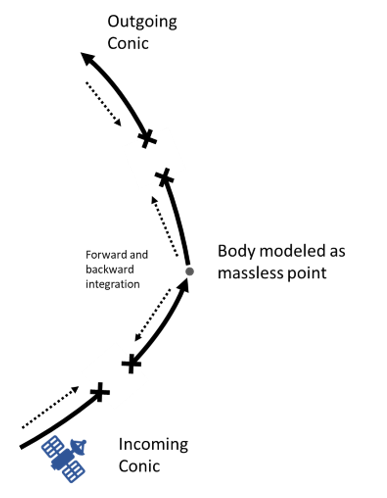
\includegraphics[width=0.5\linewidth]{Flybys_patched_conic_transcription.png}}
	\caption{\label{fig:patched_conic_transcription}Patched Conic Transcription.}
\end{figure}

\noindent In this tutorial, you will walk through how to make \ac{EMTG} model the flyby more accurately, with the spacecraft flying around the body instead of through it, while more realistically including the effects of the flyby body’s gravity during the close approach as in Figure \ref{fig:non_zsoi_transcription}.

\begin{figure}
	\centering
	\fbox{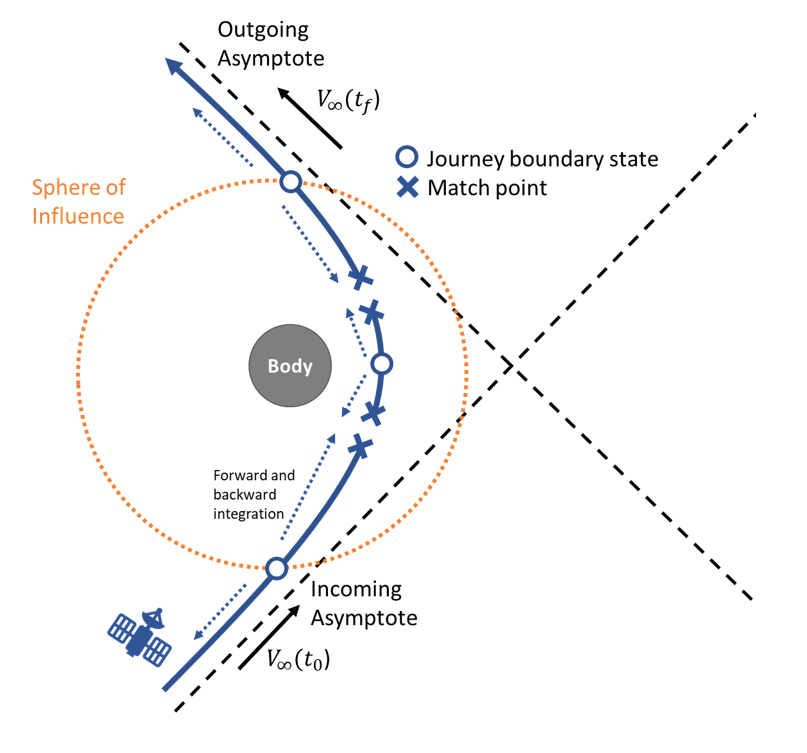
\includegraphics[width=0.8\linewidth]{Flybys_ephem_referenced_gravity_assist_multiple_shooting_transcription.png}}
	\caption{\label{fig:non_zsoi_transcription}Ephemeris-referenced Gravity-assist Multiple-shooting Transcription.}
\end{figure}

\noindent \ac{EMTG} comes with several Python scripts to help transform a \ac{ZSOI} flyby into a fully propagated flyby. First, if necessary, you can convert a multi-Phase Journey (a Journey that contains one or more bodies in the “Flyby Sequence” section of the “Journey Options” tab) to a series of single-Phase journeys (each flyby or body departure/arrival occurs at a Journey boundary) with one Python script. Then, you can convert the single-Phase-Journeys Mission to a Mission with propagated flybys using another Python script. When you finish this process, each departure, flyby, and arrival body will be represented by multiple Journeys switching the primary gravitational body (the central body) at each \ac{SOI} crossing. Table \ref{tab:emtg_conversion_scripts} summarizes this process.

\begin{table}[H]
	\begin{small}
		\begin{tabularx}{\linewidth} { >{\arraybackslash} X >{\arraybackslash} X >{\arraybackslash} X}
			\hline
			Starting \ac{EMTG}\newline Options Files & Converter & Output \ac{EMTG}\newline Options File \\
			\hline 
			Multi-Phase\newline Journey(s)\newline &  & Single-Phase Journeys with flybys \\ 
			Example:\newline Earth to Mars\newline with Venus in flyby\newline sequence & PyEMTG/Converters/convert\_to\_ single\_phase\_journeys.py & Example:\newline Journey 0: Earth to Venus \newline Journey 1: Venus to Mars\newline \\ 
			(Ephemeris-pegged boundaries) &  & (Ephemeris-pegged boundaries) \\
			\hline
			Single-Phase Journeys with flybys\newline &  & High-fidelity EMTG Mission \\
			Example:\newline Journey 0: Earth\newline to Venus\newline Journey 1: Venus\newline to Mars & PyEMTG/HighFidelity/ HighFidelityDriverFunction.py & Example:\newline Journey 0: Earth periapse to Earth SOI\newline Journey 1: Earth SOI to Venus SOI\newline Journey 2: Venus SOI to Venus periapsis\newline Journey 3: Venus periapse to Venus SOI\newline Journey 4: Venus SOI to Mars center of mass\newline \\
			(Ephemeris-pegged boundaries) &  & (Multiple Journey arrival/departure classes) \\
 			\hline
		\end{tabularx}
	\end{small}
	\caption{\label{tab:emtg_conversion_scripts}Journey Arrival Elements.}
\end{table}

%%%%%%%%%%%%%%%%%%%%%
\section{Setup}
\label{sec:setup}
%%%%%%%%%%%%%%%%%%%%%

Make a new directory for this tutorial called \texttt{Flybys} and copy and paste in the \texttt{EVM.emtgopt} file, and \texttt{hardware\_models} folders from the Journey Boundaries tutorial. Open the \texttt{EVM.emtgopt} file and change the 
paths for “Hardware library path” in the ``Spacecraft Options'' tab, and ``Working directory'' in the ``Output Options'' tab to a new \texttt{results} directory the new \texttt{Flybys} directory. Don’t forget the trailing slash in ``Hardware library path''.

\noindent You will also want to have the solution to this low-fidelity mission as an initial guess for the higher fidelity conversions, so either run mission again without changing any additional options or have the solution folder from the first EVM run in the Journey Boundaries tutorial handy. 

%%%%%%%%%%%%%%%%%%%%%
\subsection{Universe Files}
\label{sec:universe_files}
%%%%%%%%%%%%%%%%%%%%%

You need to make new Universe files before you can run the converted missions. You already have a Universe file for the Sun and for Mars, but you need them for Earth and Venus, as well, because those two bodies will now be the central bodies of Journeys. In the \texttt{EVM\_universe} directory, make two copies of the \texttt{Sun.emtg\_universe} file and call them \texttt{Earth.emtg\_universe} and \texttt{Venus.emtg\_universe}, respectively. Copy the ``\#menu of bodies'' line for the Sun from \texttt{Mars.emtg\_universe} and paste it into the Earth and Venus Universe files. Delete the ``\#menu of bodies'' line for Earth from the Earth file and the Venus line from the Venus file. Like when making the Mars universe file in the Journey Boundaries tutorial, make sure that the ID number for each body in the menu of bodies is unique. (E.g., Sun and Mercury cannot both have ID 1.) Finally, update the central body section of the Earth and Venus Universe files. 

\noindent Reference the text below for Venus.

\begin{lstlisting}
#Central body name
central_body_name Venus
#Central body SPICE ID
central_body_SPICE_ID 299
#central body radius
central_body_radius 6051.8
#gravitational constant of central body, in km^3/s^2
mu 324858.592
#characteristic length unit, in km
LU 6051.8
#angles defining the local reference frame relative to ICRF, given in degrees
#alpha0, alphadot, delta0, deltadot, W, Wdot
reference_angles 272.76 0.0 67.16 0.0 160.2 -1.4813688
#radius of the central body's sphere of influence
r_SOI 616000
#minimum safe distance from the central body
minimum_safe_distance 6351
\end{lstlisting}

\noindent Reference the text below for Earth.

\begin{lstlisting}
#Central body name
central_body_name Earth
#Central body SPICE ID
central_body_SPICE_ID 399
#central body radius
central_body_radius 6378.14
#gravitational constant of central body, in km^3/s^2
mu 398600.436296
#characteristic length unit, in km
LU 6378.14
#angles defining the local reference frame relative to ICRF, given in degrees
#alpha0, alphadot, delta0, deltadot, W, Wdot
reference_angles -90.0 -0.641 90.0 -0.557 280.147 360.9856235
#radius of the central body's sphere of influence
r_SOI 924500
#minimum safe distance from the central body
minimum_safe_distance 6678
\end{lstlisting}

\noindent When finished, you should have a working directory that looks like the one in Figure \ref{fig:working_dir_ex}. (Your results directory will be empty until later in the tutorial.) Refer to the Universe files provided with this tutorial if you are unsure about the Universe files or directory setup. You now have everything you need to convert the \texttt{EVM.emtgopt} file to higher fidelity missions.

\begin{figure}[H]
	\centering
	\fbox{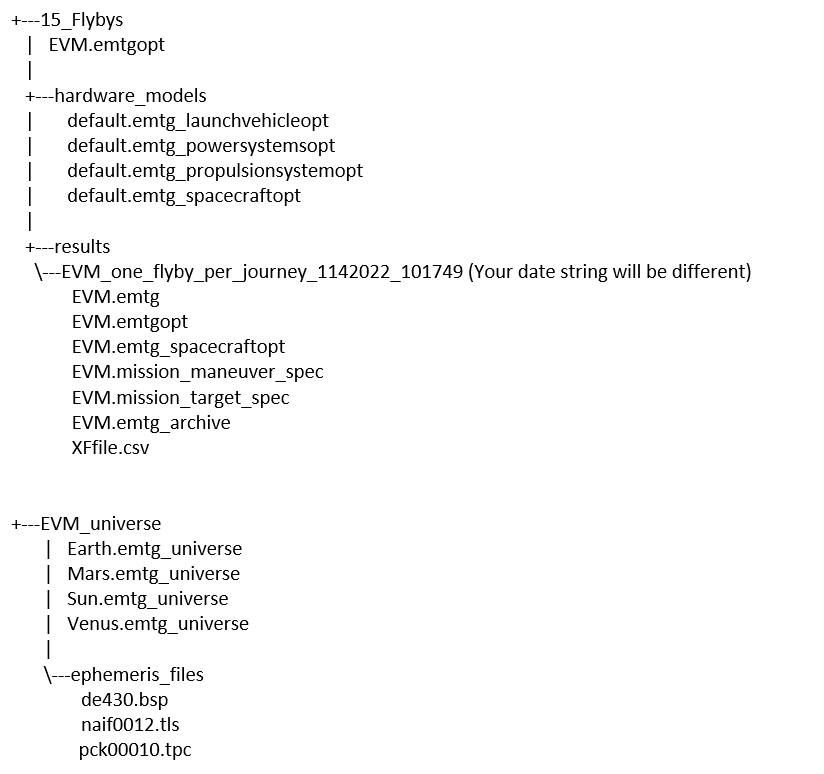
\includegraphics[width=\linewidth]{Flybys_working_directory_example.png}}
	\caption{\label{fig:working_dir_ex}Working Directory Example.}
\end{figure}

%%%%%%%%%%%%%%%%%%%%%
\section{Conversion to Single-Phase Journeys}
\label{sec:conversion_to_single_phase_journeys}
%%%%%%%%%%%%%%%%%%%%%

The first step towards a high-fidelity \ac{EMTG} mission is removing Venus from the flyby sequence and inserting it as a new Journey departure and arrival point. This is easy to do with PyEMTG, but you’re going to take advantage of a Python converter script to show how it can be done automatically. One advantage of using the Python converter script is that it automatically populates the initial guess for the new Journey structure with the values from the old Journey structure, including appropriately renaming the relevant decision variables. As a result, if the Journey structure is the only thing that is changed, \ac{EMTG} should produce exactly the same trajectory with either Journey structure.

\noindent The script is located in your \ac{EMTG} repository at \texttt{EMTG/PyEMTG/Converters/convert\_to\_single\_ phase\_journeys.py}. Open this file with a text editor like Notepad++ or VSCode. Notice that there is a \texttt{sys.path.append} line near the top of the file in the imports section. This path needs to point to your PyEMTG directory. If you installed EMTG somewhere other than what is shown, update this line so that the script has the correct path to your PyEMTG directory. Save the file. Now, you will perform the first conversion to single-phase Journeys.

\noindent Open a terminal and execute the script with Python, providing two arguments: one for the path to the EMTG options file (\texttt{EVM.emtgopt}) and the other for the path to the EVM solution file (\texttt{EVM.emtg}). As an example (all in one line),
\texttt{python C:\textbackslash <EMTG-FOLDER>\textbackslash emtg\textbackslash PyEMTG\textbackslash Converters \textbackslash convert\_to\_single\_phase\_journeys.py C:\textbackslash <PATH-TO-WORKING-DIR>\textbackslash EVM.emtgopt C:\textbackslash <PATH-\newline TO-WORKING-DIR>\textbackslash results\textbackslash EVM\_DATE\_TIME\textbackslash EVM.emtg}

\noindent You should now have a file called \texttt{EVM\_singlePhase.emtgopt} alongside your \texttt{EVM.emtgopt} file. Open \texttt{EVM\_singlePhase.emtgopt} in PyEMTG. You should have two Journeys called ``Earth\_to\_Mar s\_phase0'' and ``Earth\_to\_Mars\_phase1'' with the Journey arrival and departures shown in Table \ref{tab:single_phase_journey_state_types}. The full list of settings is shown in Figure \ref{fig:single_phase_journey_options}. Phase 0 refers to the Earth-to-Venus trajectory, and phase 1 refers to the Venus-to-Mars trajectory. Note that this does not change the Mars arrival state to the free point Journey arrival state you saw in the Journey Boundaries tutorial. 

\begin{table}[H]
	\begin{small}
		\begin{tabularx}{\linewidth} { >{\arraybackslash} X >{\arraybackslash} X >{\arraybackslash} X >{\arraybackslash} X >{\arraybackslash} X}
			\hline
			Journey Name & Journey\newline Departure Type & Journey\newline Departure Class & Journey\newline Arrival Type & Journey\newline Arrival Class \\
			\hline 
			Earth\_to\_Mars\_\newline phase0 & 0: launch or\newline direct insertion & 0: Ephemeris-pegged & 2: Intercept with bounded V\_infinity & 0: Ephemeris-pegged \\ 
			 & & & & \\
			Earth\_to\_Mars\_\newline phase1 & 3: flyby & 0:Ephemeris-pegged & 2: Insertion into parking orbit\newline (use chemical Isp) & 0: Ephemeris-pegged \\ 
 			\hline
		\end{tabularx}
	\end{small}
	\caption{\label{tab:single_phase_journey_state_types}Single Phase Journey State Types.}
\end{table}

\begin{figure}[H]
	\centering
	\fbox{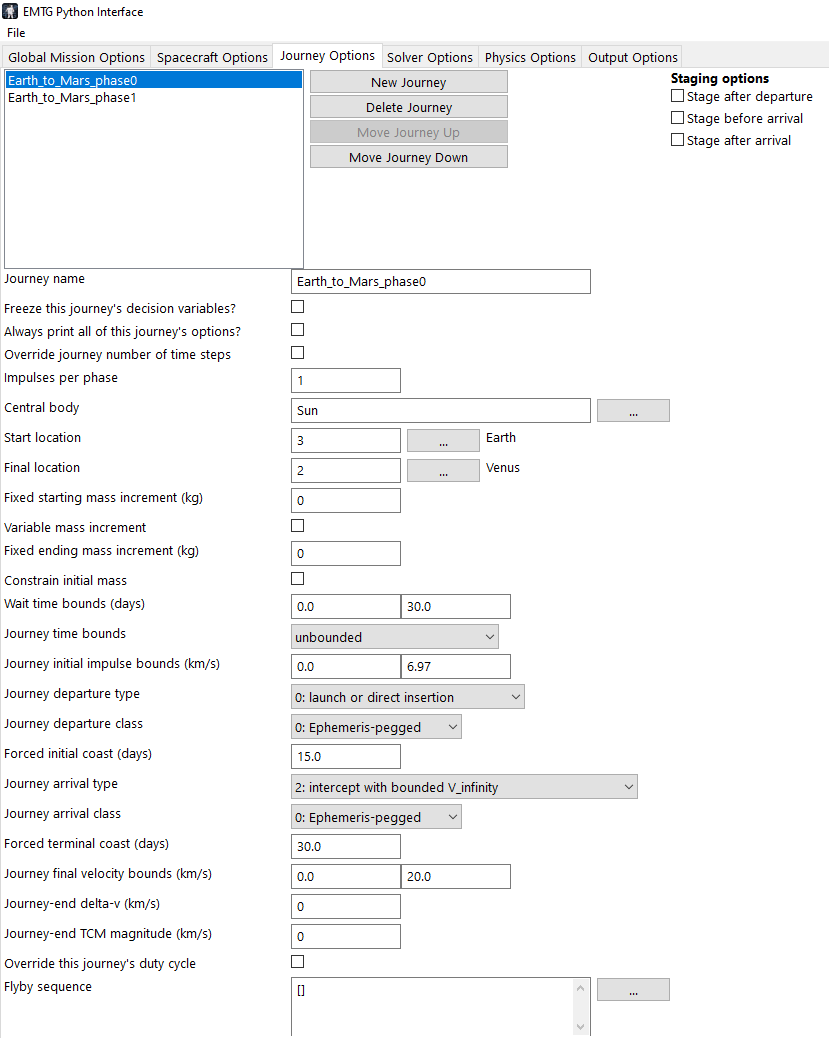
\includegraphics[width=\linewidth]{Flybys_single_phase_journey_options.png}}
	\caption{\label{fig:single_phase_journey_options}Single Phase Journey Options.}
\end{figure}

%%%%%%%%%%%%%%%%%%%%%
\subsection{Seeding}
\label{sec:seeding}
%%%%%%%%%%%%%%%%%%%%%

Open the \texttt{EVM\_singlePhase.emtgopt} in a text editor or select “File” -\textgreater “open file in editor” (Ctrl+e) in PyEMTG. Scroll down to the Journeys section and look for the entry ``\#trial decision vector'' at the end of each section of Journey options. The trial decision vector for each Journey has been ``seeded'' or filled in using the solution from \texttt{EVM.emtg} as an initial guess. The names of the decision variables may be difficult to parse at first due to the lack of spaces, but you will probably be able to understand at least vaguely what a lot of the variables mean.

\noindent \knownissuelabel{NOTE: PyEMTG may not open the file in a text editor if the file is associated with another program.}{text_editor_issue}

\noindent You can also seed the new \ac{EMTG} options file you just created with the results from another trial by using the ``Seed MBH?'' option in the ``Solver Options'' tab of the \acs{GUI}. Seeding provides a starting point for the optimizer and can help the optimizer find a solution more quickly than starting from a random guess. Switch to the ``Solver Options'' tab and check this box to reveal the ``Trial decision vector or initial guess'' button, which you can use to select previous results (i.e., a previous .emtg file) as an initial guess for this mission. These settings are shown in Figure \ref{fig:seed_mbh}.
 
\noindent \textit{NOTE:} The conversion script already provided a good initial guess and populated the appropriate sections of \texttt{EVM\_singlePhase.emtgopt}. The new single-Phase Mission decision vector is not the same as the original Mission, and the conversion script has provided initial guesses for each new variable. Using the ``Seed MBH?'' box here and selecting the old \texttt{EVM.emtg} as the seed will NOT provide a guess for every decision variable in the new single-Phase Mission, and you will get \ac{EMTG} console output such as:

\noindent \texttt{Initial guess missing value for: j0p0MGAnDSMsEphemerisPeggedIntercept: V\_infinity\_x}

\begin{figure}
	\centering
	\fbox{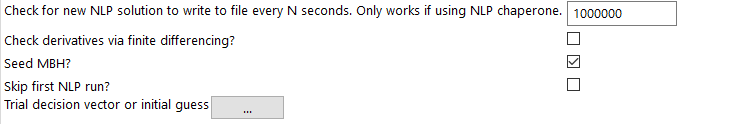
\includegraphics[width=\linewidth]{Flybys_seed_mbh.png}}
	\caption{\label{fig:seed_mbh}Seed \acs{MBH}.}
\end{figure}

%%%%%%%%%%%%%%%%%%%%%
\subsection{Run the Mission}
\label{sec:run_the_mission_single_phase}
%%%%%%%%%%%%%%%%%%%%%

Run the file (Ctrl+r) and note that the \ac{EMTG} terminal output reads something like,

\noindent \texttt{NLP incumbent point and exit point are feasible and incumbent point is superior to exit point.}

\noindent Or

\noindent \texttt{NLP incumbent point was infeasible but less infeasible than the exit point.}

\noindent after loading the \acs{SPICE} files. Depending on your mission and the solution provided to the conversion script, the output of the single-phase script may or may not already have a feasible initial guess. (If the \texttt{EVM.emtg} file you provided to the conversion script was feasible, the new Mission should be feasible, too. You can check this directly by switching to the ``Solver Options'' tab, selecting ``Evaluate trialX'' in ``Inner-loop Solver Mode'', then running \ac{EMTG}. If your output looks like that shown in Figure \ref{fig:evaluate_trialx_output} with the text ``Decision vector is feasible'', the initial guess is feasible. (Do not expect the exact numbers to be the same because \ac{EMTG} is a stochastic optimizer.) Let’s increase the fidelity of this mission further.

\begin{figure}[H]
	\centering
	\fbox{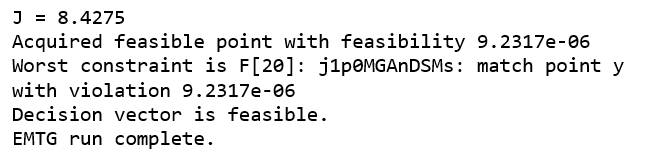
\includegraphics[width=0.7\linewidth]{Flybys_evaluate_trialx_output.png}}
	\caption{\label{fig:evaluate_trialx_output}Evaluate TrialX Output.}
\end{figure}

%%%%%%%%%%%%%%%%%%%%%
\section{Conversion to High-fidelity Mission}
\label{sec:conversion_to_single_phase_journeys}
%%%%%%%%%%%%%%%%%%%%%

The high-fidelity conversion script takes an \ac{EMTG} options file with single-Phase Journeys and solution as input. It’s located in \texttt{EMTG/PyEMTG/HighFidelity/HighFidelityDriverFunction.py}. Before running it, you need to check another system path command in the file \texttt{EMTG/PyEMTG/HighFide lity/HighFidelityJourney.py}. As before, open the file in a text editor and check that the \texttt{sys.path.append} line near the top of the file points to your PyEMTG folder, or the Python import statements will not work correctly.

\noindent Now open \texttt{HighFidelityDriverFunction.py} in a text editor. This conversion script does not use command-line arguments. Instead, scroll down to the ``\texttt{if \_\_name\_\_ == "\_\_main\_\_":}'' section. Change the \texttt{originalOptionsFile} variable to point to the single-Phase Journeys \ac{EMTG} options file. Change the \texttt{originalMissionsFile} variable to point to the single-Phase Journeys \ac{EMTG} solution file, and the \texttt{outputFilePath} variable to point to the directory where you wish to save the high-fidelity \ac{EMTG} options file. This section in your file should now look something like the one in Figure \ref{fig:highfidelitydriverfunction_example}.

\noindent Save and run the script using the terminal command:

\noindent \texttt{python EMTG/PyEMTG/HighFidelity/HighFidelityDriverFunction.py} 

\begin{figure}[H]
	\centering
	\fbox{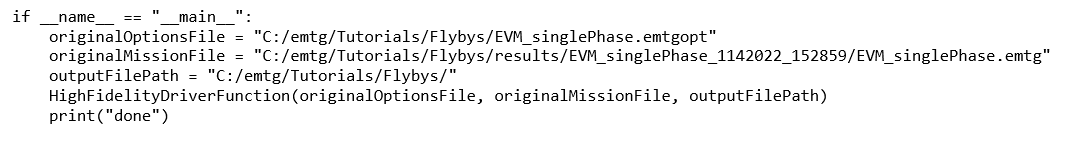
\includegraphics[width=\linewidth]{Flybys_highfidelitydriverfunction_example.png}}
	\caption{\label{fig:highfidelitydriverfunction_example}HighFidelityDriverFunction.py Example.}
\end{figure}

\noindent A new file called \texttt{HighFidelity.emtgopt} should be created in the directory you specified in \texttt{outputFilePath}. Open it with PyEMTG.

\noindent Notice that you now have several more Journeys. The \ac{EMTG} mission now proceeds from Earth periapse to Earth \acs{SOI} to Venus \acs{SOI} to Venus periapse to Venus \acs{SOI} to Mars. The converter has also included the \acs{SOI} radius from the Earth and Venus Universe files when defining the ephemeris-referenced arrival states. Table \ref{tab:high_fidelity_journey_state_types} shows the new Journey configuration.

\begin{table}[H]
	\begin{small}
		\begin{tabularx}{\linewidth} { >{\arraybackslash} X >{\arraybackslash} X >{\arraybackslash} X >{\arraybackslash} X >{\arraybackslash} X}
			\hline
			Journey Name & Journey\newline Departure Type & Journey\newline Departure Class & Journey\newline Arrival Type & Journey\newline Arrival Class \\
			\hline 
			EarthLaunch & 0: launch or\newline direct insertion & 3: Periapse & 2: Intercept with bounded V\_infinity & 2: Ephemeris-referenced \\
			 & & & & \\
			Earth\_to\_Mars\_\newline phase0 & 2: free direct departure & 1: Free point & 2: Intercept with bounded V\_infinity & 0: Ephemeris-referenced \\ 
			 & & & & \\
			VenusGAi & 2: free direct departure & 1: Free point & 2: Intercept with bounded V\_infinity & 3: Periapse \\
			 & & & & \\
			Venus GAo & 2: free direct departure & 1: Free point & 2: Intercept with bounded V\_infinity & 2: Ephemeris-referenced \\
			 & & & & \\
			Earth\_to\_Mars\_\newline phase1 & 3: free direct departure & 0: Free point & 2: Insertion into parking orbit\newline (use chemical Isp) & 0: Ephemeris-pegged \\ 
 			\hline
		\end{tabularx}
	\end{small}
	\caption{\label{tab:high_fidelity_journey_state_types}High Fidelity Journey State Types.}
\end{table}

\noindent Note that neither of the conversion scripts changed the Mars ephemeris-pegged arrival to the more realistic Mars \acs{SOI} to Mars free point arrival orbit you created in the Journey Boundaries tutorial. You’ll need to do that yourself. Since it was covered previously, you won’t update the high-fidelity mission here. The high-fidelity conversion script only converts ephemeris-pegged launches and ephemeris-pegged flybys to propagated trajectories.

\noindent Like with the single-Phase conversion script, the high-fidelity flyby conversion script also generates initial guesses for the new decision variables, and you can examine them in the new \texttt{HighFidelity.e mtgopt} file. Unlike the results of the single-Phase conversion, though, you should not necessarily expect the high-fidelity decision variables to produce a feasible solution without optimization, even if the starting low-fidelity \ac{EMTG} case was feasible. However, the initial guess is usually quite good, though the quality of the initial guess tends to degrade as the flyby speed decreases (i.e., for near-parabolic flybys).


%%%%%%%%%%%%%%%%%%%%%
\subsection{Flyby Sensitivity}
\label{sec:flyby_sensitivity}
%%%%%%%%%%%%%%%%%%%%%

Select the ``VenusGAi'' (Venus gravity assist in) journey. An example is shown in Figure \ref{fig:high_fidelity_journey_options}. Notice at the bottom of the Journey options, there is a section of options related to the match point and integration step size. Between each Journey departure and arrival, \ac{EMTG} places a ``match point'' (sometimes also known as a ``break point'') where the state integrated forwards from current Journey departure state and the state integrated backwards from the current Journey arrival state need to match, see Figure \ref{fig:non_zsoi_transcription}. Matching states near a gravity assist periapse is tricky because of the sensitive dynamics, and it can be difficult for \acs{SNOPT} to converge if the match point is not ideally placed.

\noindent To deal with this, the conversion script overrode the default match point location (halfway in time between Journey arrival and departure) and placed the match point close to periapse. This results in a value for ``Where do you want to place the match point? (fraction)'' of 0.9 (90\% of the way from the SOI to periapse or equivalently 10\% of the way from periapse to the \acs{SOI}). The conversion script has also reduced the integration step size backwards from periapse to 60 seconds rather than 600 seconds at the \acs{SOI} forwards because the spacecraft is moving much faster near periapse than near the \acs{SOI} boundary. Switch to the ``VenusGAo'' (Venus gravity assist out) Journey and notice that these values are reversed. The values pre-populated in these fields by the conversion script are rules of thumb and should be overridden by the user as appropriate for each unique scenario. These changes can be seen in Figure \ref{fig:gravity_assist_options}.

\begin{figure}[H]
	\centering
	\fbox{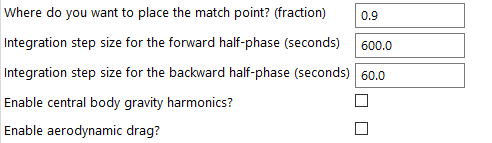
\includegraphics[width=0.8\linewidth]{Flybys_gravity_assist_match_point_options.png}}
	\caption{\label{fig:gravity_assist_options}Incoming Gravity Assist Match Point Options.}
\end{figure}

\begin{figure}[H]
	\centering
	\fbox{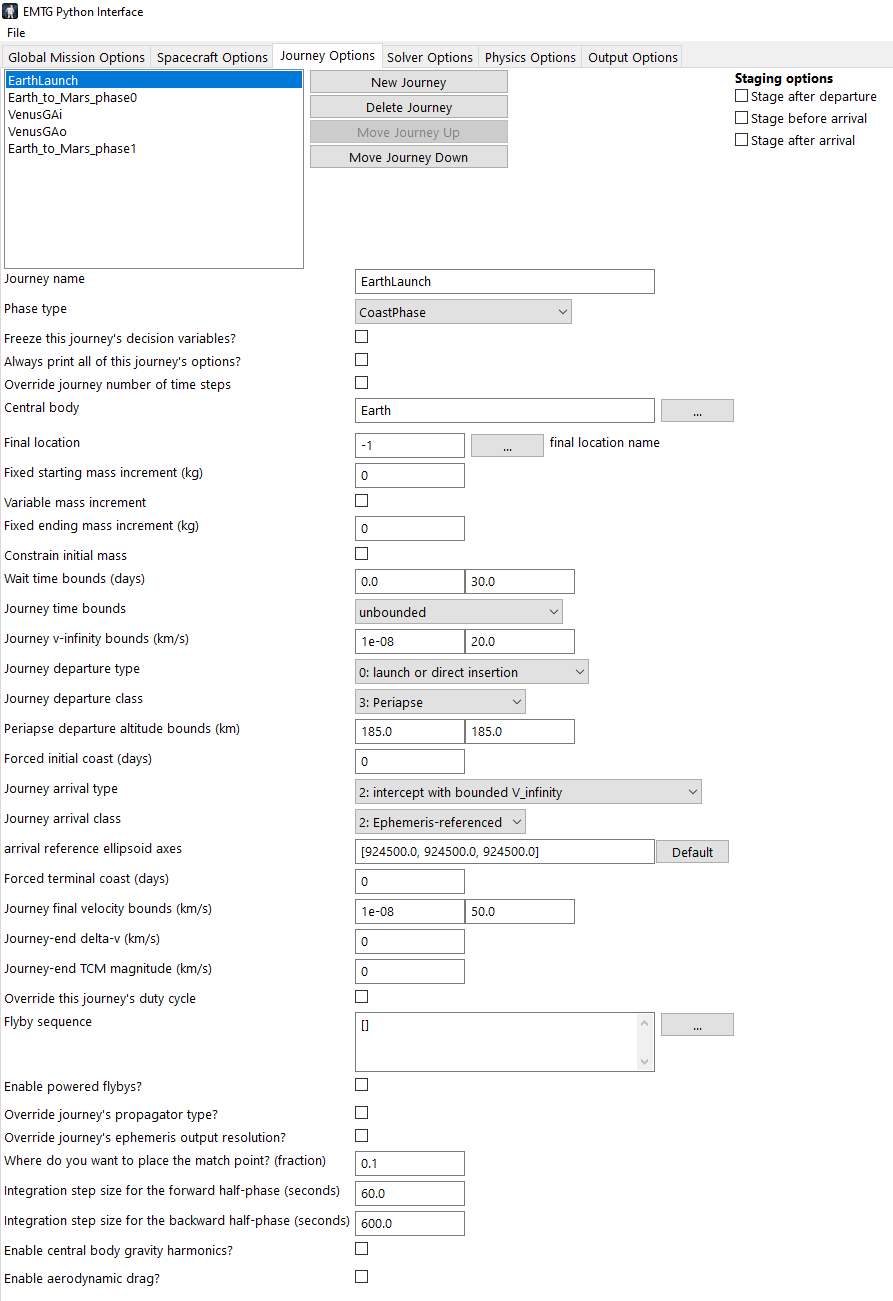
\includegraphics[width=\linewidth]{Flybys_high_fidelity_journey_options.png}}
	\caption{\label{fig:high_fidelity_journey_options}High Fidelity Journey Options Tab.}
\end{figure}


%%%%%%%%%%%%%%%%%%%%%
\subsection{Periapse State Representation}
\label{sec:periapse_state_representation}
%%%%%%%%%%%%%%%%%%%%%

Switch to the ``Physics Options'' tab. At the bottom of the PyEMTG window are additional options to specify how \ac{EMTG} defines states in the multiple shooting problem. The ``PeriapseBoundary state representation'' option specifies the flyby periapse state definition. The default is ``SphericalRADEC'' for spherical right-ascension and declination. Click the drop-down list to see the other state representations available to define the periapse state. Sometimes switching the periapse state encoding can make it easier for \acs{SNOPT} to converge on a solution.

\noindent It is possible to switch this state representation and define additional flyby constraints such as B-plane targets using this feature as shown in Figure \ref{fig:state_representation_settings}. This is beyond the scope of this tutorial.

\begin{figure}[H]
	\centering
	\fbox{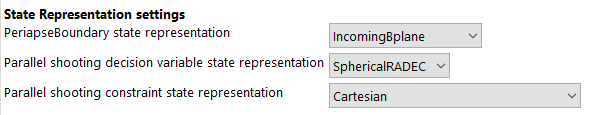
\includegraphics[width=0.9\linewidth]{Flybys_state_representation_settings.png}}
	\caption{\label{fig:state_representation_settings}Example of Different State Representation Settings.}
\end{figure}

%%%%%%%%%%%%%%%%%%%%%
\subsection{Run the Mission}
\label{sec:run_the_mission_high_fidelity}
%%%%%%%%%%%%%%%%%%%%%

Run the high-fidelity mission (Ctrl + r) with \acs{MBH} using the initial guess created by the high-fidelity conversion script encoded automatically in the generated \ac{EMTG} options file. You should not expect the initial guess to be feasible. However, the guess should help \ac{EMTG} find a solution much faster than running this high-fidelity script without a guess due to the larger decision vector, larger constraint vector, and increased sensitivity of the problem. In practice, \ac{EMTG} can often converge to a feasible high-fidelity trajectory based on this process with a single \acs{NLP} solve (i.e., no \acs{MBH}). Try it yourself and see! 

\noindent This concludes the tutorial on high-fidelity flybys. You can now convert a low-fidelity but easy-to-solve \ac{EMTG} options file using a ``Flyby sequence'' to a sequence of Journeys which more accurately model the spacecraft’s trajectory. In the Force Models tutorial, you will learn how to increase the realism further by adding additional gravitational bodies and other perturbing forces.


\end{document}